\documentclass[9pt]{IEEEtran}

\usepackage[english]{babel}
\usepackage{graphicx}
\usepackage{epstopdf}
\usepackage{fancyhdr}
\usepackage{amsmath}
\usepackage{amsthm}
\usepackage{amssymb}
\usepackage{url}
\usepackage{array}
\usepackage{textcomp}
\usepackage{listings}
\usepackage{hyperref}
\usepackage{xcolor}
\usepackage{colortbl}
\usepackage{float}
\usepackage{gensymb}
\usepackage{longtable}
\usepackage{supertabular}
\usepackage{multicol}

\usepackage[utf8x]{inputenc}

\usepackage[T1]{fontenc}
\usepackage{lmodern}{}
\input{glyphtounicode}
\pdfgentounicode=1

\graphicspath{{./figures/}}
\DeclareGraphicsExtensions{.pdf,.png,.jpg,.eps}

% correct bad hyphenation here
\hyphenation{op-tical net-works semi-conduc-tor trig-gs}

% ============================================================================================

\title{\vspace{0ex}
Mean-Shift tracking}

\author{Marko Medved\vspace{-4.0ex}}

% ============================================================================================

\begin{document}

\maketitle

\section{Introduction}
In this assignment, the mean shift method was implemented and used to develop a tracker, which was 
evaluated on the VOT14 dataset. The model's performance was analyzed under different parameter settings. 
The tracker was further enhanced by incorporating additional weights into the histogram, with the weights
 adjusted based on the background characteristics of the tracked object.

\section{Experiments}
\subsection{Mean shift mode seeking on the given example}
The Mean Shift method was tested with various parameters to evaluate its performance. 
The kernel size, which defines the region for the calculation of the current step,
 was adjusted. Larger 
kernels led to faster convergence, but excessively large or small kernels
 prevented convergence to the local maximum. Different starting positions were tested, showing
  that starting points in low-probability areas prevented movement, and for multi-modal 
  functions, the starting point determined which maximum the algorithm would reach.

Three convergence criteria were evaluated: (1) step size, stopping when movement is under 
one pixel; (2) Euclidean distance, halting when consecutive positions differ by less than 
two units; and (3) change in probability, stopping when the probability shift is minimal. 
The sub-pixel step size was the most consistent but slowest, while the probability-based
 criterion sometimes caused premature convergence if early changes were small. 
 Figure~\ref{fig:mode_seeking} shows how these parameters influenced convergence. Note 
 that each color represents a different starting position.

\begin{figure}[h]
    \centering
    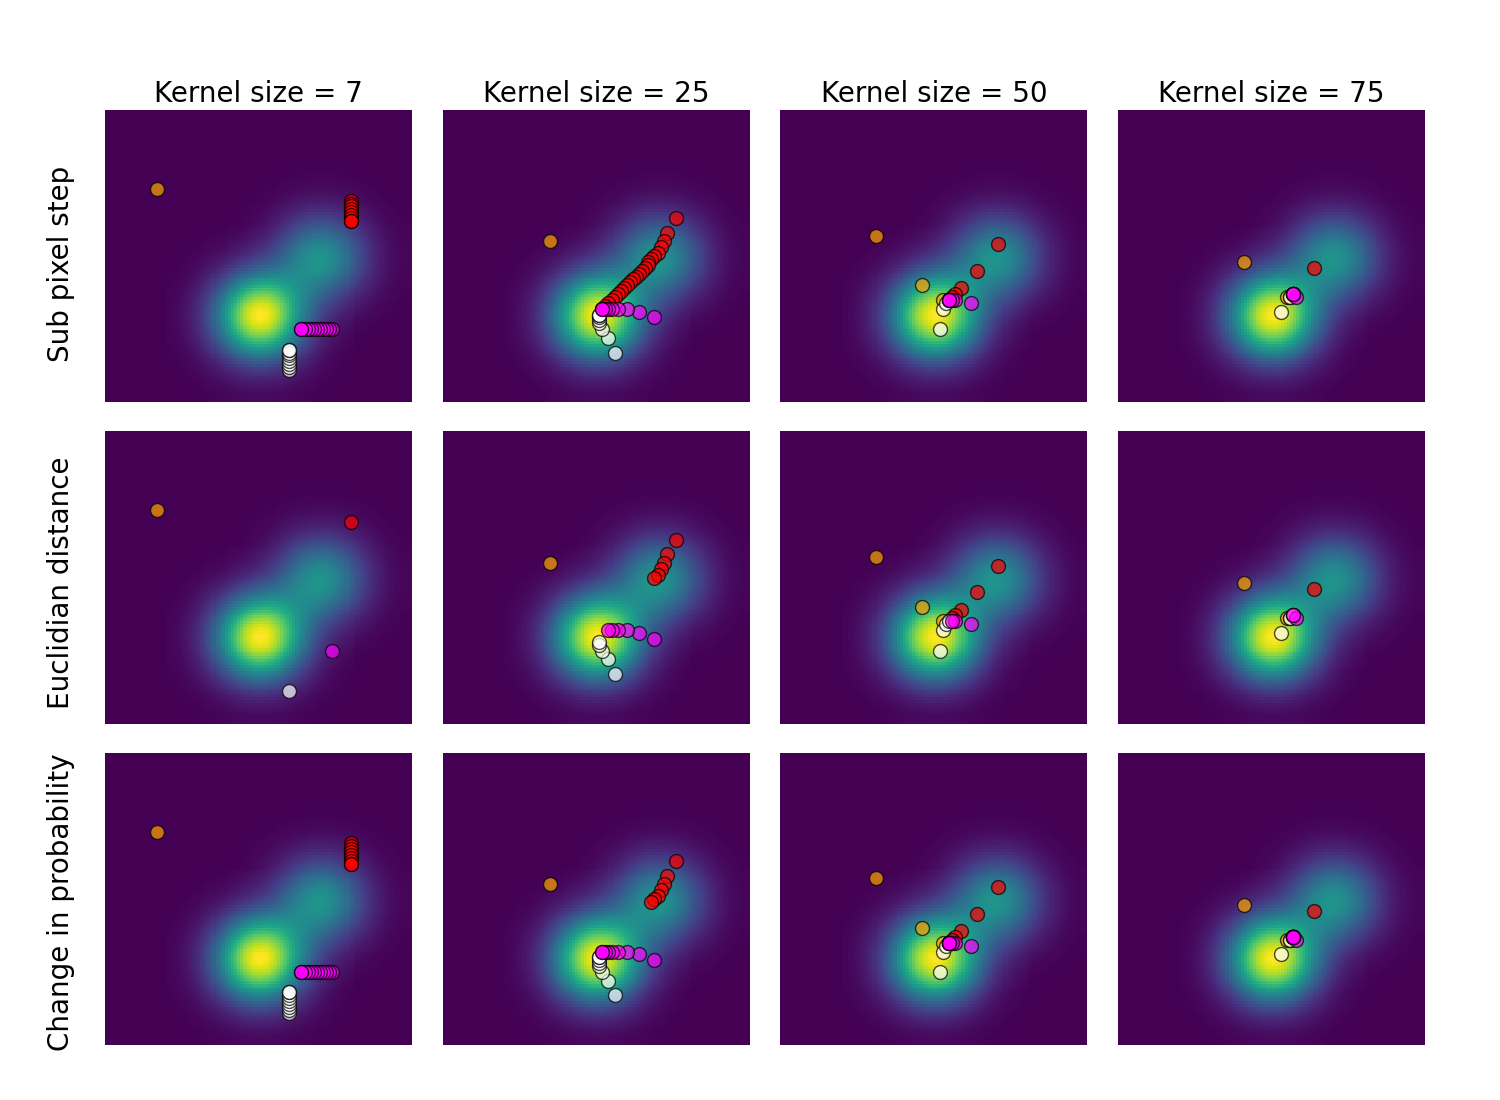
\includegraphics[width=0.99\columnwidth]{figures/mode_seeking.png}
    \caption{Comparison of the mean shift method with different kernel sizes, convergence
    criteria and starting positions}
    \label{fig:mode_seeking}
\end{figure}


\subsection{Mean shift mode seeking on custom examples}
The algorithm was then tested on three custom functions, shown in 
Figure~\ref{fig:mode_seeking2}. In these tests, the sub-pixel convergence criterion
 was used, and the kernel size was set to 25. For each function, four different 
 starting positions were evaluated. The first function is a Gaussian distribution, 
 where the algorithm consistently converges to the global maximum, provided the 
 starting point is not in a region with near-zero probability. The second example 
 is the Laplacian of Gaussian (the Mexican hat function), which has multiple local
  maxima. Here, the convergence outcome strongly depends on the starting position.
   The final example is a small section of the Julian Alps (around 46° North and 
   14° East). Due to the presence of many local maxima, the starting position 
   determines which peak the algorithm will ascend to. 

\begin{figure}[h]
  \centering
  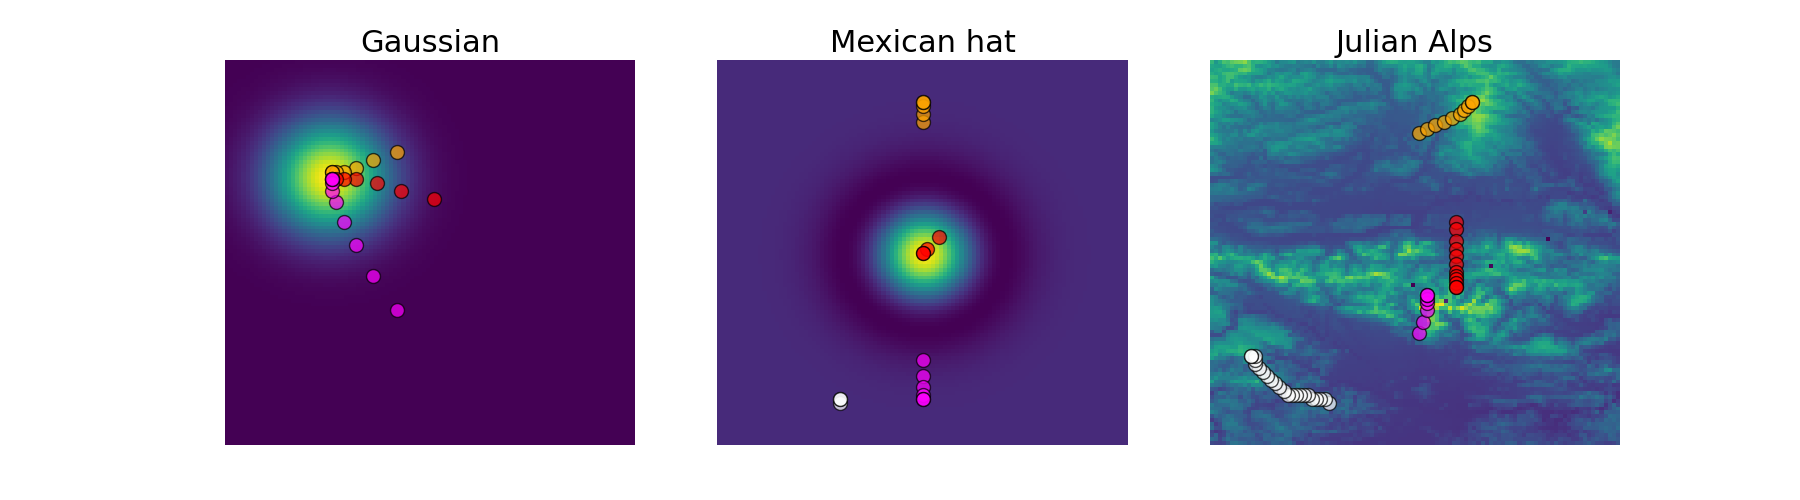
\includegraphics[width=0.99\columnwidth]{figures/mode_seeking2.png}
  \caption{Comparison of the mean shift method on different functions}
  \label{fig:mode_seeking2}
\end{figure}

\subsection{Basic tracker implementation}
The tracker was implemented and tested on the entire VOT 2014 dataset. 
The number of failures and the tracking speed (measured on my personal laptop)
 are summarized in Table~\ref{tab:basic_tracker_results}. Overall, the tracker 
 failed a total of 33 times across the dataset. While the tracker performs reliably
  in most cases, it struggles more with certain sequences, such as hand2, fish1,
   torus, and tunnel. The reasons behind these failures will be explored in detail in the next section. 

\begin{table}[h]
  \centering
  \caption{Basic Tracker Results}
  \setlength{\tabcolsep}{3pt}
  \begin{tabular}{l|c|c||l|c|c}
  \hline
  \textbf{Sequence} & \textbf{Failures} & \textbf{Speed} & \textbf{Sequence} & \textbf{Failures} & \textbf{Speed} \\ 
  \hline
  ball       & 1 & 1823 FPS & david     & 1 & 1042 FPS \\ 
  basketball & 0 & 510 FPS  & diving    & 0 & 1328 FPS \\ 
  bicycle    & 1 & 1047 FPS & drunk     & 1 & 700 FPS  \\ 
  bolt       & 2 & 1425 FPS & fernando  & 2 & 358 FPS  \\ 
  car        & 0 & 2017 FPS & fish1     & 3 & 1571 FPS \\ 
  fish2      & 1 & 1224 FPS & motocross & 2 & 504 FPS  \\ 
  gymnastics & 0 & 1667 FPS & polarbear & 0 & 2020 FPS \\ 
  hand1      & 2 & 923 FPS  & skating   & 1 & 1098 FPS \\ 
  hand2      & 5 & 2610 FPS & sphere    & 0 & 1285 FPS \\ 
  jogging    & 1 & 1704 FPS & sunshade  & 0 & 928 FPS  \\ 
  surfing    & 0 & 3179 FPS & torus     & 3 & 1170 FPS \\ 
  trellis    & 2 & 1449 FPS & tunnel    & 4 & 2684 FPS \\ 
  woman      & 1 & 2525 FPS &           &   &          \\ 
  \hline
  \end{tabular}
  \label{tab:basic_tracker_results}
  \end{table}
  
  
  \subsection{Failure cases discussion}
  Figure~\ref{fig:failures} shows the cases where the tracker experienced the most failures.
   In the fish1 and hand2 sequences, failures occurred due to similar color distributions 
   between the tracked object and the background, making it hard to detect movement.
    In the torus and tunnel sequences, scale changes added complexity: in torus, object 
    rotation altered the color distribution, and in tunnel, the motorbike’s decreasing size 
    led to an inaccurate bounding box.

  These failure cases suggest two potential improvements: addressing scale changes by testing
   different template scales and minimizing the influence of the background. The latter is 
   discussed in the final section.

  \begin{figure}[h]
    \centering
    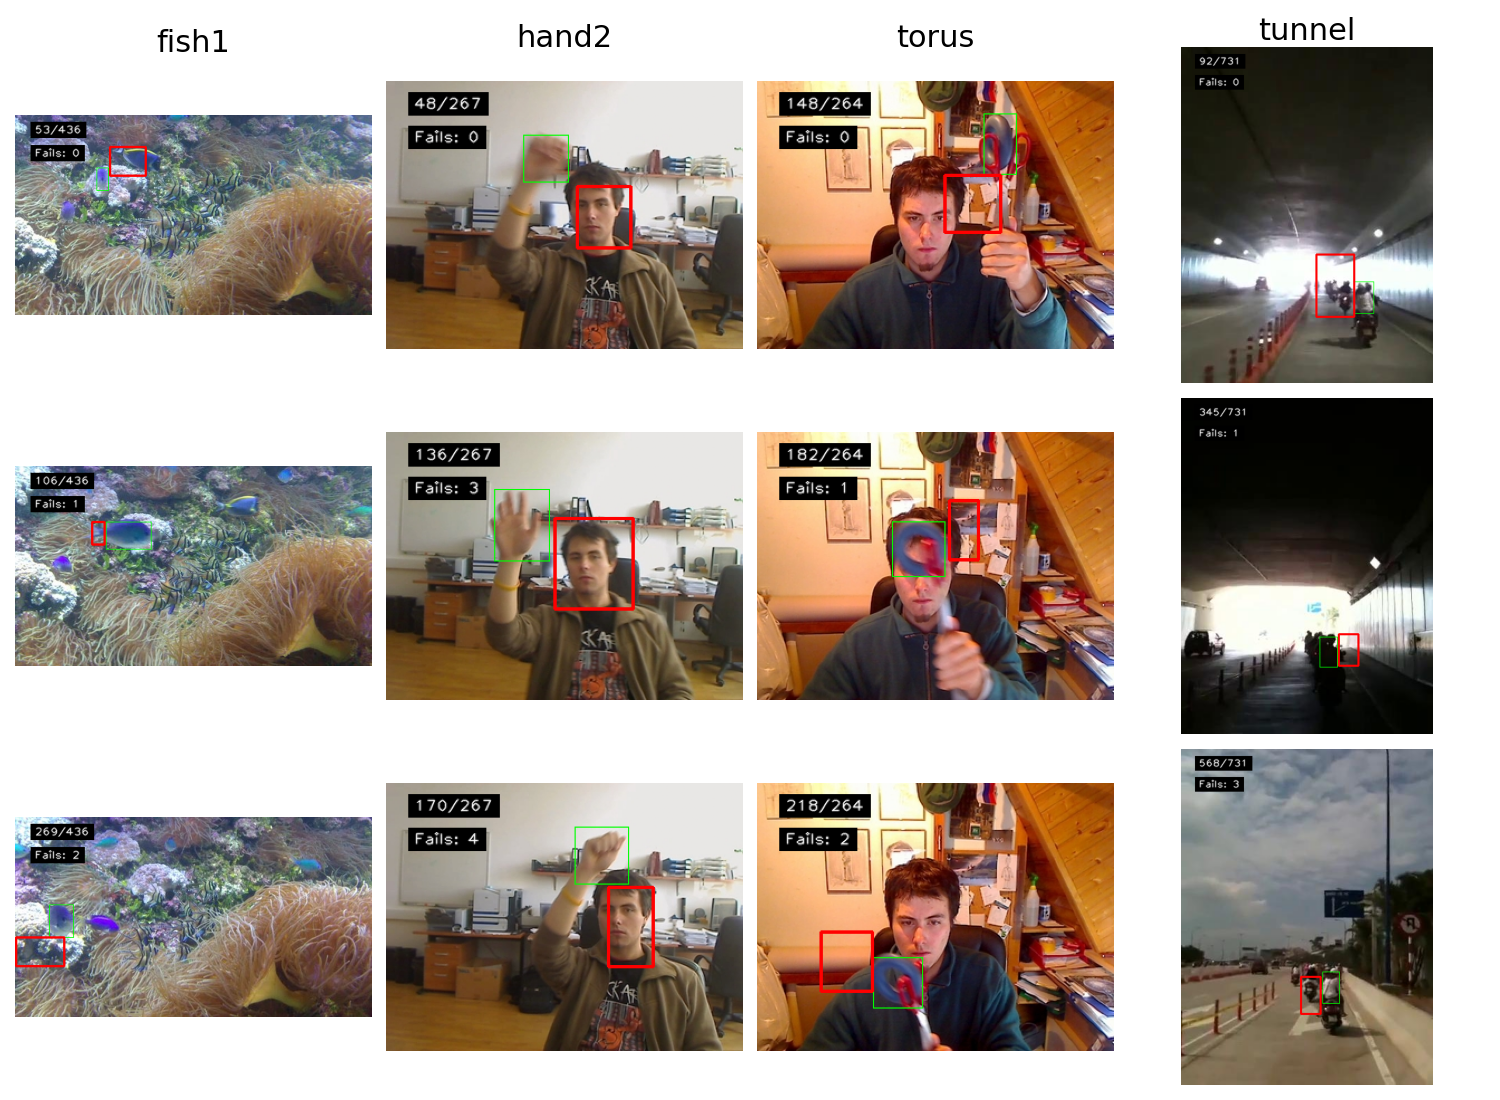
\includegraphics[width=0.99\columnwidth]{figures/failures.png}
    \caption{Mean shift tracker failure cases}
    \label{fig:failures}
  \end{figure}

\subsection{Parameter tuning}
Four key parameters were tested: $\sigma$ (kernel size), histogram bin count, 
iterations per frame, and $\alpha$ (template update rate). The algorithm was 
evaluated for all combinations of 4 bin counts, 5 kernel sizes, 3 iteration values,
 and 6 update rates.

 To determine the optimal number of iterations and bins, the results were averaged with respect to 
  these two parameters (Figure~\ref{fig:params1}). The data shows that using only one iteration 
  significantly reduces performance, while 10 and 20 iterations produce similar results. Since
   the average performance is very similar between 10 and 20 iterations, the 20-iteration version
    will be used for further evaluation, as it produced the top 3 best single results, including 
    the best result with 25 failures across the entire dataset.

    Regarding the number of bins, 8 and 16 bins outperform the others and 
     deliver a really similar performance. 
    However, since the top 7 single results were produced by the 16-bin version, this version will
     be used for further evaluation.


 \begin{figure}[h]
  \centering
  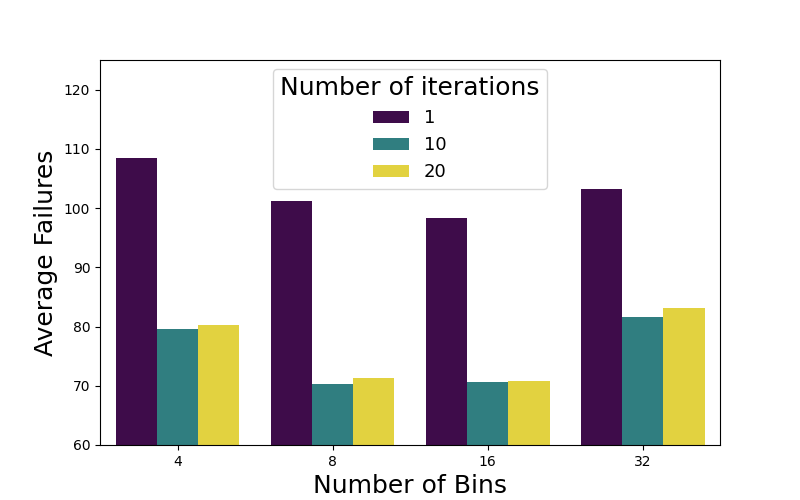
\includegraphics[width=0.95\columnwidth]{figures/nbins_niters.png}
  \caption{Performance of the means shift tracker with different numbers of bins and numbers of
  iterations}
  \label{fig:params1}
\end{figure}

To determine the best values for $\sigma$ and $\alpha$, we refer to Figure~\ref{fig:params2}. 
The optimal $\sigma$ could be 0.5 or 1, but we choose 1 since it produced the top 2 single
 results. For $\alpha$, performance is similar across the range from 0 to 0.01, but 0.001 appears
  to slightly outperform the others. We can interpret that, while updating the template can help, 
  it should be performed really slowly.
\begin{figure}[h]
  \centering
  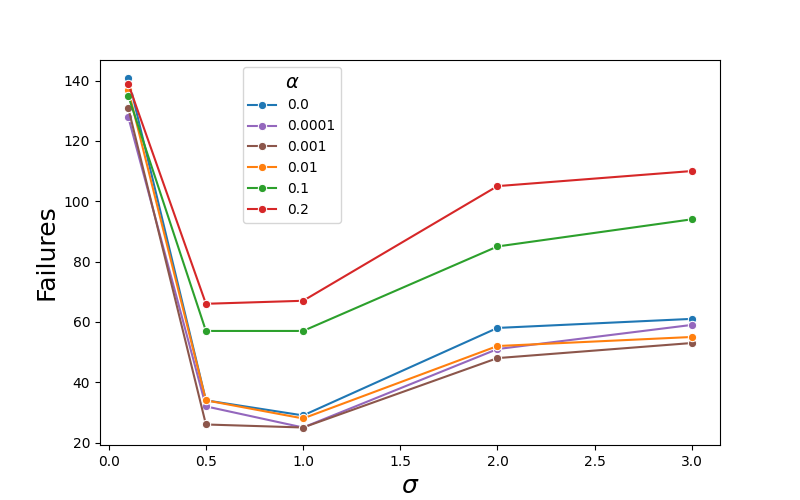
\includegraphics[width=0.99\columnwidth]{figures/sigma_alpha.png}
  \caption{Performance of the means shift tracker with different kernel sizes and update rate
  parameters}
  \label{fig:params2}
\end{figure}

\subsection{Feature selection by accounting for the background in different color spaces}
To mitigate the influence of the background, the method applied smaller weights to the regions in the histogram where
 the background color predominated. The tracker was also evaluated using five different color spaces. Additionally,
  a new parameter was introduced: the size of the background area. In the results, the optimal size of the background area 
  for each color space will be taken for evaluation.

Table~\ref{tab:color_spaces_results} presents the number of failures across the entire dataset for each color 
space using the optimal parameters, showing an improvement over the basic 
method(except for the YCrCb color space) . Note that by using the HSV color 
space, which performed best on the entire dataset,
 the performance
 on the most challenging videos (hand2, fish1, torus, and tunnel) improved, with the number of failures
  reduced to 4, 1, 0, and 3, respectively. 

   \begin{table}[h]
    \centering
    \caption{Performance of the improved tracker across different color spaces.}
    \begin{tabular}{lcc}
    \hline
    \textbf{Color space} & \textbf{Failures} & \textbf{Average Speed [FPS]} \\ 
    \hline
    RGB                 & 19                & 981                  \\ 
    LAB                 & 21                & 831                  \\ 
    HSV                 & 16                & 1002                 \\ 
    YCrCb               & 26                & 1230                 \\ 
    BGR                 & 19                & 1646                 \\ 
    \hline
    \end{tabular}

    \label{tab:color_spaces_results}
    \end{table}
    

\section{Conclusion}
In this assignment, the mean shift algorithm and tracker were implemented.
 The analysis identified the problematic test sequences and explored the potential reasons for failure.
  The results demonstrated that the tracker’s performance can be significantly improved by carefully tuning the 
  parameters and incorporating background information into the model.
\bibliographystyle{IEEEtran}
\bibliography{bibliography}

\end{document}
